\chapter{Ανίχνευση προσώπων}\label{ch:facedetection}
Η επιστημονική περιοχή της ανίχνευσης αντικειμένου μπορεί να χωριστεί
σε τρεις επιμέρους ανεξάρτητες διαδικασίες.
\begin{itemize}
    \item Εντοπισμός πιθανών περιοχών αντικειμένου/ων
    \item Ταξινόμηση αντικειμένου
    \item Προσδιορισμός θέσης αντικειμένου
\end{itemize}


H διαδικασία του εντοπισμού των περιοχών αντικειμένων αφορά την εύρεση των περιοχών
εντός μιας εικόνας όπου είναι πιθανό να υπάρχουν αντικείμενα. Πιο συγκεκριμένα, αφορά τον προσδιορισμό
του συνόλου των εικονοστοιχείων εκείνων τα οποία με μια γρήγορη επεξεργασία δίνουν
μεγάλη πιθανότητα να εμπεριέχουν ένα αντικέιμενο. αναπαριστούν αντικείμενα μέσα σε

Η ταξινόμηση αντικειμένου αφορά τον προσδιορισμό της κλάσσης του αντικειμένου που
έχει προσδιοριστεί. Η διαδικασία της ταξινόμησης απαιτεί την εξαγωγή διάφορων
χαρακτηριστών από την εικόνα και επεξεργασία αυτών με κάποιο αλγόριθμο ταξινόμησης
για τον συμπερασμο της κλασσης του αντικειμενου.

Ο τελικός προσδιορισμός της θέσης του αντικειμένου εντός της εικόνας μπορεί να γίνει σε
τρία επίπεδα: α) σε επίπεδο εικόνας, β) σε επίπεδο περιγράμματος γ) σε επίπεδο παραθύρου
(βλ. Σχήμα \ref{fig:bee}).

\begin{figure}[htp]
    \centering
    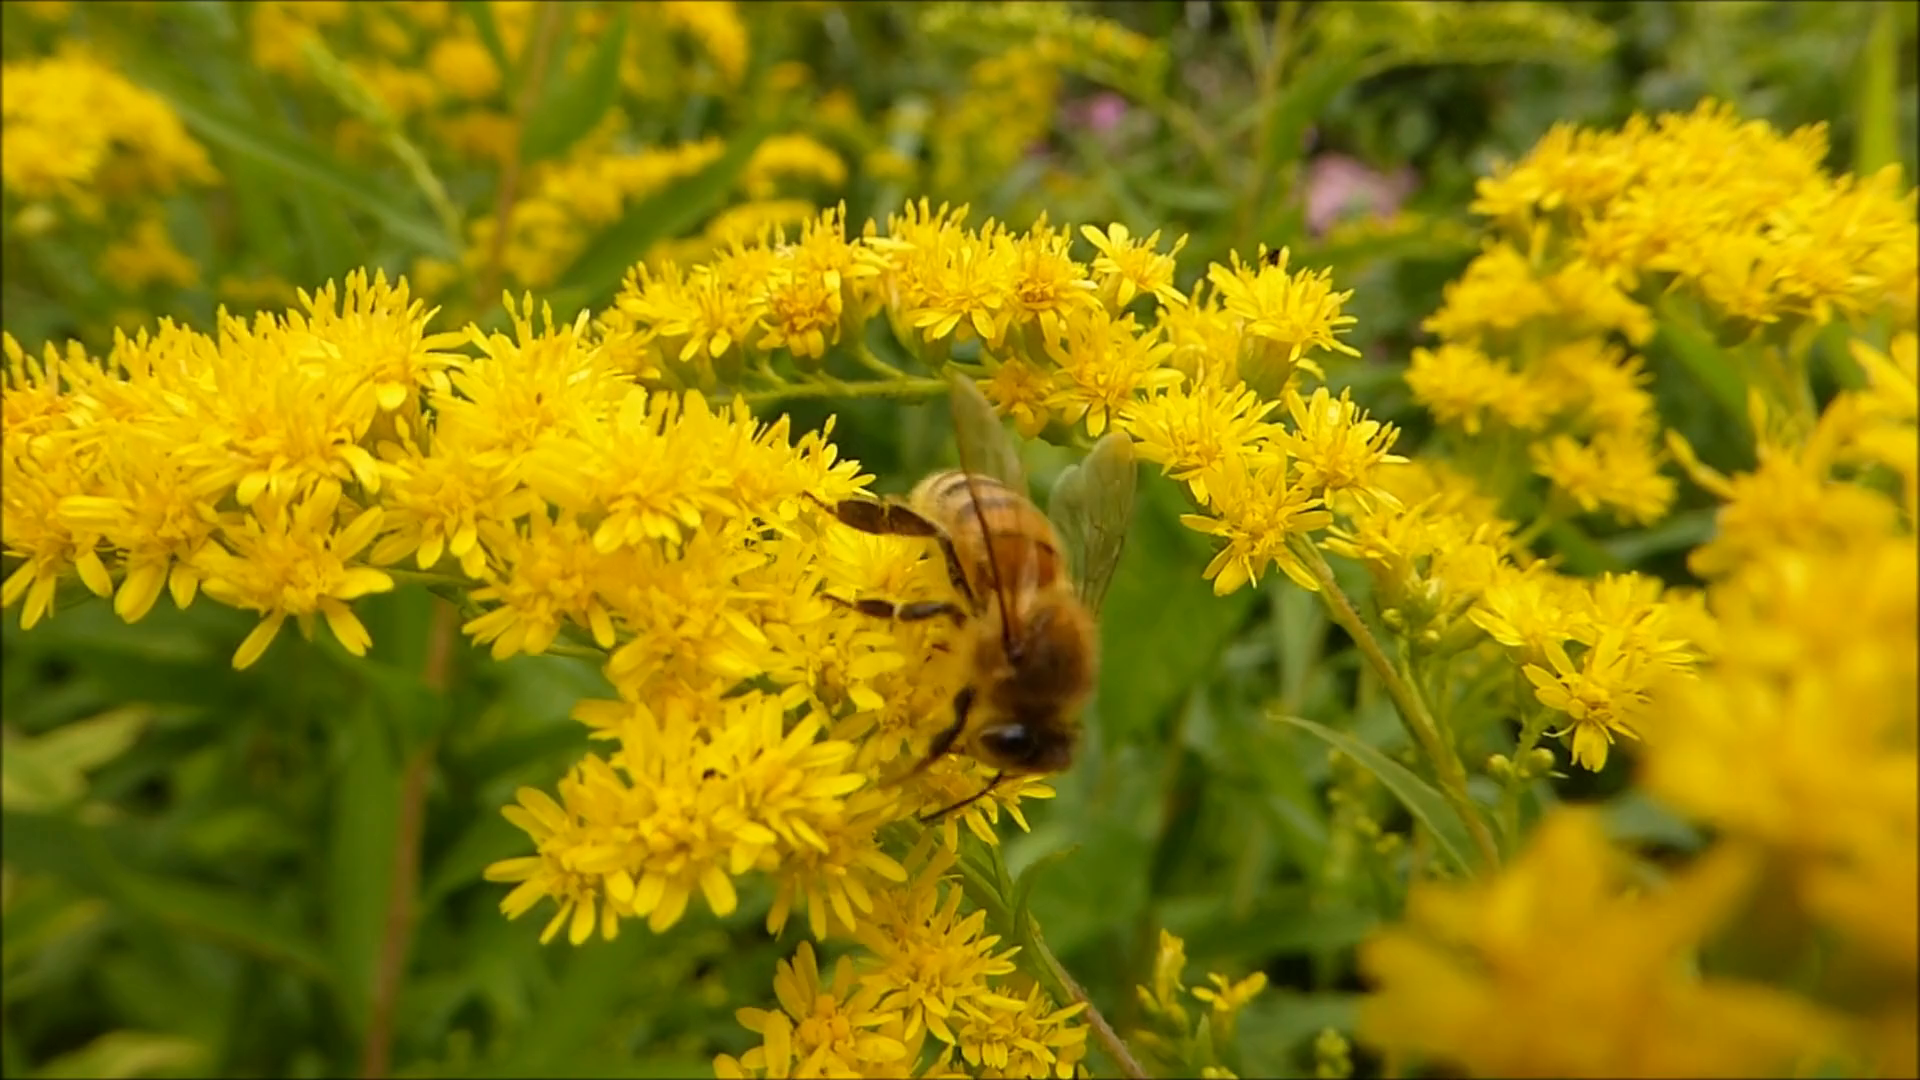
\includegraphics[width=.49\textwidth]{../figures/bee.png}\hfill
    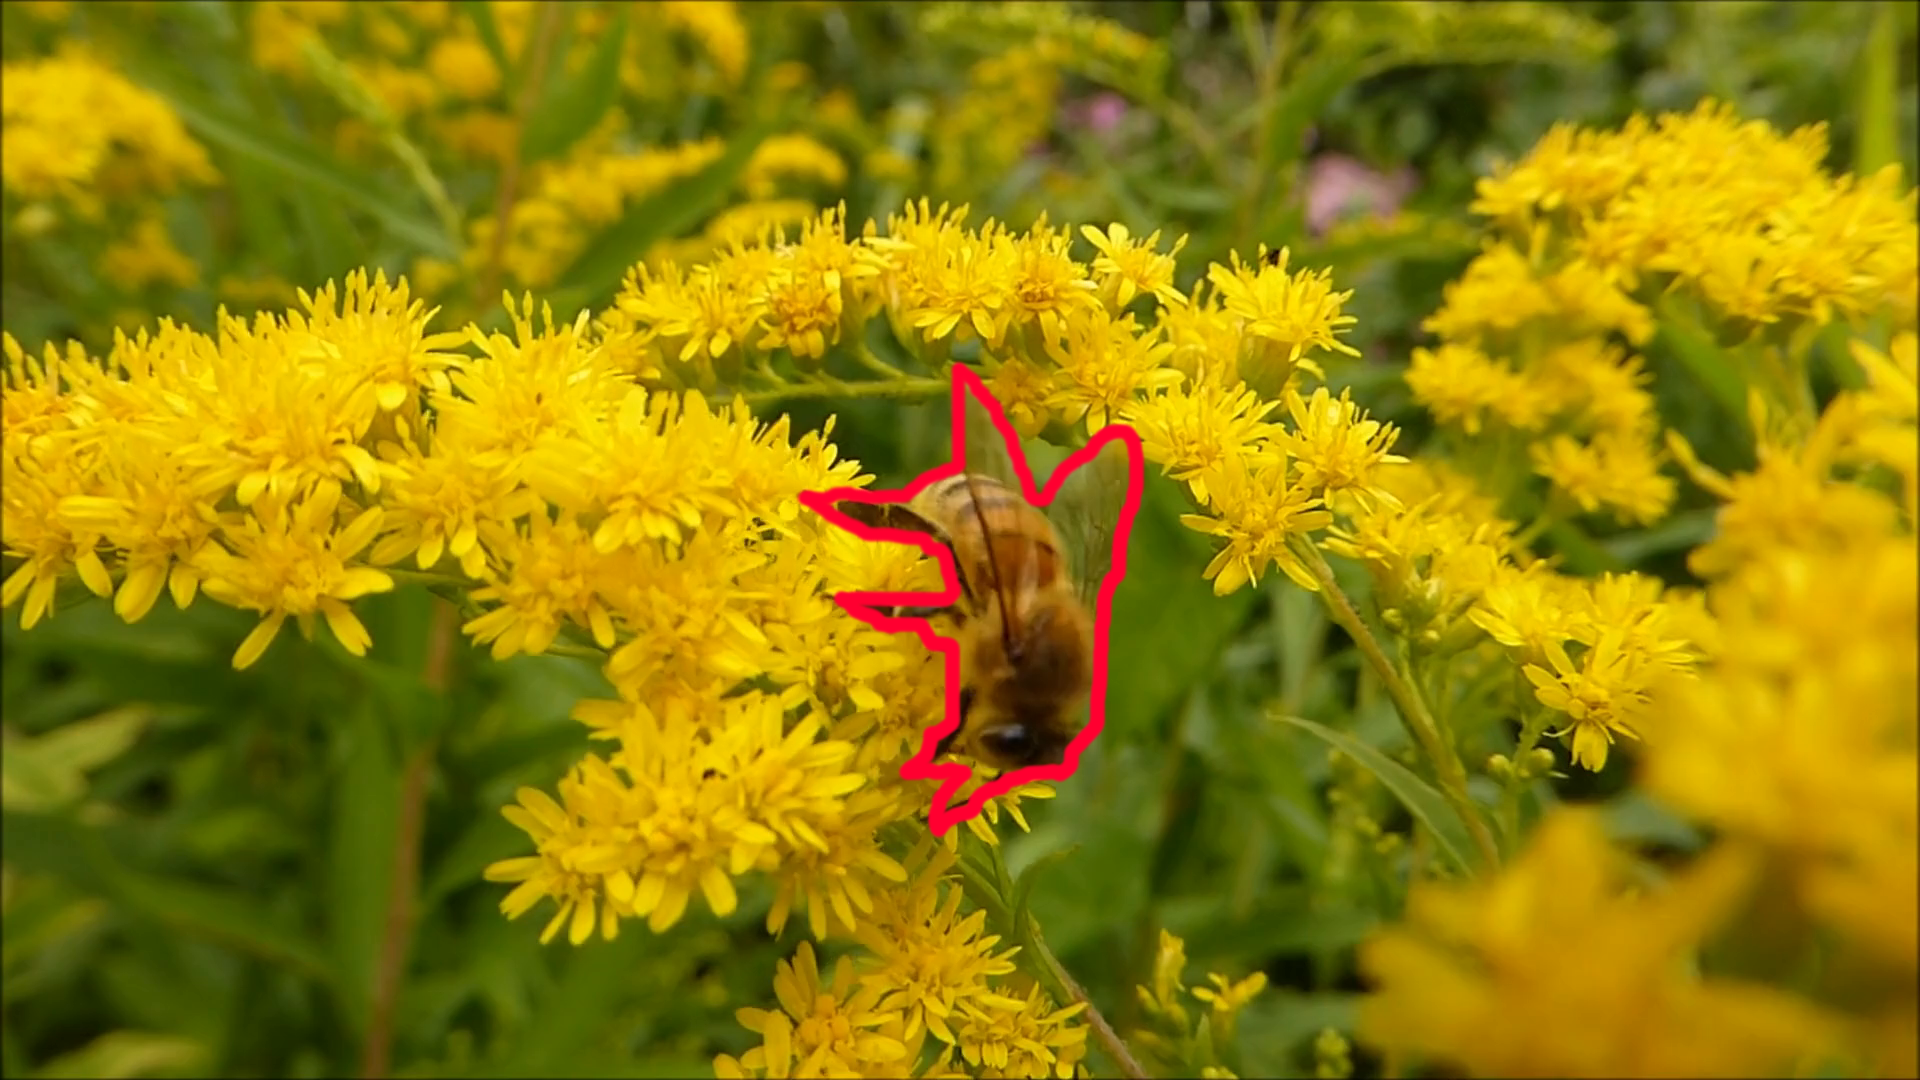
\includegraphics[width=.49\textwidth]{../figures/beescissors.png}\hfill
    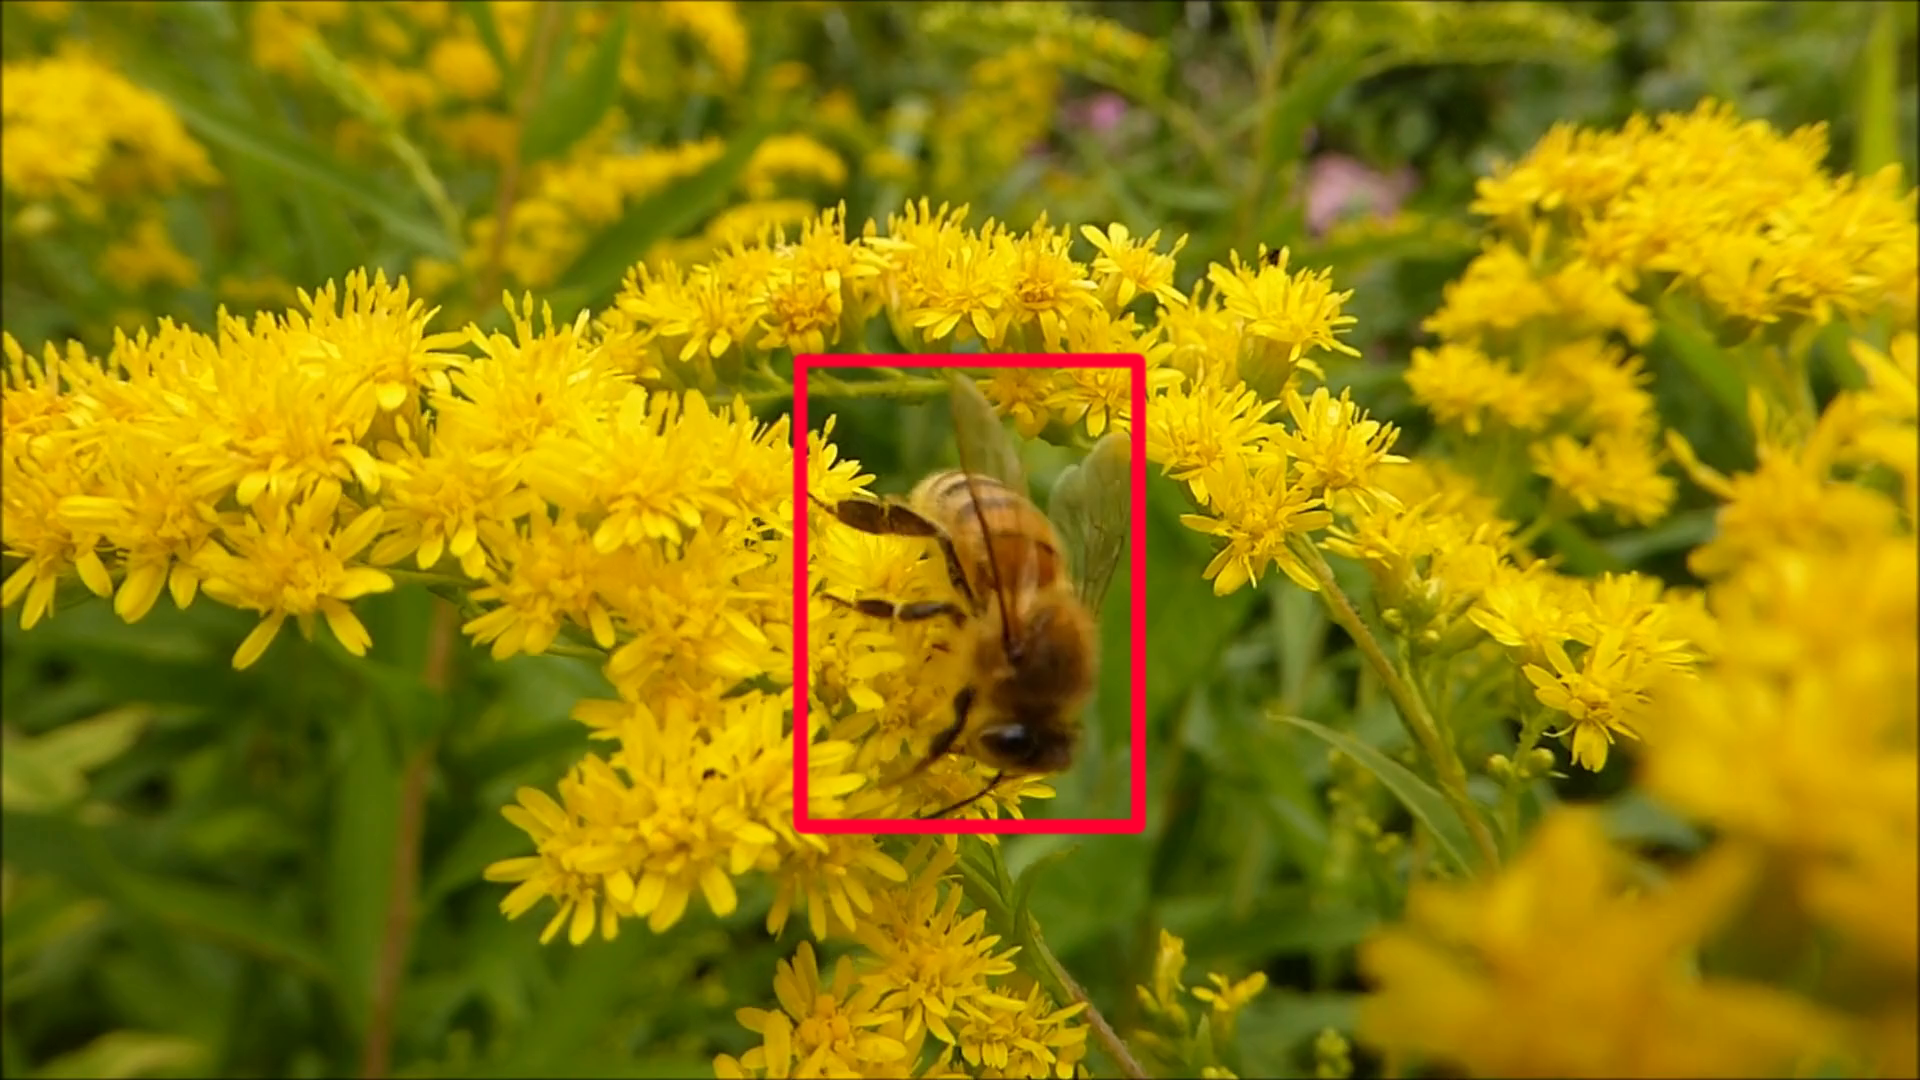
\includegraphics[width=.48\textwidth]{../figures/beebbox.png}\hfill

    \caption{α) σε επίπεδο εικόνας, β) σε επίπεδο περιγράμματος γ) σε επίπεδο παραθύρου.}
    \label{fig:bee}

\end{figure}

Στη συνέχεια του κειμένου της παρούσας διπλωματικής όταν αναφερόμαστε στον όρο
ανίχνευση αντικειμένου θα αναφερόμαστε στην ανίχνευση σε επίπεδο παραθύρου.

Η ανίχνευση προσώπου αποτελεί μια υποπεριοχή της ανίχνευσης αντικείμενου. Επομένως
η μεθοδολογία που ακολουθείται είναι όμοια με αυτή που περιγράψαμε ανωτέρω. Ειδικότερα,
η ανίχνευση προσώπου παρουσιάζει μια ευκολία σε σχέση με την ανίχνευση κλάσης αντικειμένου
με την έννοια ότι κάθε πρόσωπο έχει συγκεκριμένα και καθολικά χαρακτηριστικά στο
σύνολο των ανθρώπων. Συνεπώς, η ανίχνευση προσώπου δεν αφορά το γενικότερο πρόβλημα
του εντοπισμού της κλάσης ενός αντικειμένου αλλά το υποπρόβλημα του εντοπισμού
-εντός μια εικόνας- μιας και μόνον κλάσης αντικειμένου (του προσώπου) με αυστηρώς
προσδιορισμένα χαρακτηριστικά.

Παρακάτω θα κάνουμε μια σύντομη περιγραφή των βασικότερων μεθόδων αναγνώρισης
προσώπου που έχουν χρησιμοποιηθεί έως σήμερα.

\section{Συνοπτική παρουσίαση βασικών μεθόδων αναγνώρισης προσώπων}\label{sec:facedetmethods}

In recent years, virtualization has become an important consideration and has
gained popularity in many different areas such as server consolidation, cloud
computing, corporate data centers, and the academic world. This is largely due
to an increase in hardware performance of about ten fold in the past decade, the
need to reduce the capital and operational cost to the minimum~\cite{Graziano},
and the desire to run multiple operating systems in a single host.

\begin{flushright}
  \emph{``A virtual machine is taken to be an efficient,\\
        isolated duplicate of the real
        machine."}~\cite{DBLP:journals/cacm/PopekG74}


  Gerald J. Popek and Robert P. Goldberg
\end{flushright}


\subsection{Η μέθοδος Rowley, Baluja και Kanade~\cite{Rowley:1998:NNF:275341.275344}}

To 1998 οι \emph{Rowley, Baluja και Kanade} περιέγραψαν μια μέθοδο για την αναγνώριση
προσώπων βασισμένη στο συνδιασμό αποτελεσμάτων από νευρωνικά δίκτυα. Στην εικόνα
δοκιμάζεται ένα σετ απο φίλτρα βασισμένα σε νευρωνικά δίκτυα. Στη συνέχεια τα
αποτελέσματα επεξεργάζονται από ένα διαμεσολαβιτή και συνδιάζονται. Πιο συγκεκριμένα
η μέθοδος αποτελείται από 2 βήματα:

\begin{description}\label{item:rowley}
  \item[Βήμα 1] \hfill \\
    Στο βήμα αυτο επιλεγεται αρχικα ενα παράθυρο μεγέθους 20x20 από την αρχική εικόνα.
    Το παράθυρο αυτό υπόκειται μια προεργασία για την ισοστάθμιση της έντασης του
    χρώματος, την αντίθεση κ.α. και στη συνέχεια δίνεται ως είσοδο σε ένα ή και
    περισσότερα (προεκπαιδευμένα) νευρωνικά δίκτυα. Τα δίκτυα αυτά υπολογίζουν κάποια
    συγκεκριμένα χαρακτηριστικά που αφορούν τα πρόσωπα (πχ μύτη, μάτια, στόμα) και
    αποφασίζουν αν στο παράθυρο αυτό υπάρχει ή όχι πρόσωπο. Η εικόνα σαρώνεται
    ολόκληρη σε παράθυρα μεγέθους 20x20 τα οποία ακολοθούν την παραπάνω ροή.
    Το μέγεθος του παραθύρου αυξάνεται σταδιακά με ένα προκαθορισμένο βάρος για
    εντοπίσει πρόσωπα μεγαλύτερα του προαναφερθέντος μεγέθους.
  \item[Βήμα 2] \hfill \\
    Το παρόν βήμα αποτελείται από δύο υπο-βήματα. Αφενός συλλέγονται τα επιμέρους
    αποτελέσματα του κάθε νευρωικού δικτύου και με βάση μια ευριστική απορρίπτονται
    κάποιες λανθασμένες (false positive) προβλέψεις. Αφετέρου, συνδιάζονται τα
    αποτελέσματα από όλα τα επιμέρους νευρωνικά δίκτυα και χρησιμοποιώντας κάποια
    άλλη ευριστική παράγονται οι τελικές προβλέψεις του αλγορίθμου για τα πρόσωπα.
\end{description}

Βάση μετρήσεων η παραπάνω μέθοδος μπορεί να επιτύχει ποσοστά επιτυχούς αναγνώρισης
προσώπων μεταξύ $77.9\% - 90.3\%$ -με ένα ασφαλή αριθμό λαναθασμένων προβλέψεων-
ανάλογα με τις ευριστικές μεθόδους που χρησιμοποιούνται.

\subsection{H μέθοδος SNow(Sparse Network of Winnows)~\cite{Yang00asnow-based}}

Αργότερα, το \emph{2000} oι \emph{Yang, Roth} και \emph{Ahuja} πρότειναν μια νέα
μέθοδο βασισμένη στην αρχιτεκτονική εκμάθησης \emph{SNoW}~\cite{Roth98learningto}~\cite{CCRR99}.
Η αρχιτεκτονική αυτή -\emph{SNoW}- (Sparse Network of Winnows)
είναι στην πραγματικότητα ένα δίκτυο από γραμμικές συναρτήσεις που χρησιμοποιούν
τον κανόνα Winnow~\cite{Littlestone:1988:LQI:639961.639994} και επιτρέπει την
ανίχνευση προσώπων με διαφορετικά χαρακτηριστικά, σε δοαφορετικές θέσεις και
στάσεις και με διαφορές στις φωτιστικές συνθήκες. Το σύστημα αυτό είναι ειδικά
σχεδιασμένο για μάθηση σε τομείς στους οποίους ο δυνητικός αριθμός των
χαρακτηριστικών που συμμετέχουν στις αποφάσεις είναι πολύ μεγάλο, αλλά μπορεί να
είναι άγνωστο a priori.

Η διαδικασία της αναγνώρησης προσώπου είναι όμοια με αυτή των \emph{Rowley, Baluja και Kanade}
όπου η εικόνα σαρώνεται αρχικά σε παράθυρα μεγέθους 20x20 και το μέγεθος αυτό
αυξάνεται σε κάθε επανάληψη κατά μια σταθερή, προκαθορισμένη τιμή $(1.2)$. Η
διαδικασία αυτή επαναλαμβάνεται 10 φορές. Σε κάθε επανάληψη το τρέχον παράθυρο
από την εικόνα δίνεται ως είσοδο στο προεκπαιδευμένο δίκτυο SNoW το οποίο λαμβάνει
την απόφαση για την ύπαρξη ή όχι προσώπου υπολογίζοντας κάθε φορά ένα διαφορετικό
αριθμό χαρακτηριστικών.

Η μέθοδος αυτή μπορεί να επιτύγχανει ποσοστά επιτυχίας κοντά στο $93\%$.

\section{H μέθοδος Viola-Jones}\label{sec:violjon}

O αλγόριθμος των Viola-Jones~\cite{Viola01rapidobject} υπήρξε τομή στο πεδίο
της ανίχνευσης αντικειμένων σε εικόνες. Ουσιαστικά δημιούργησε την πρώτη
υποδομή ανίχνευσης αντικειμένων η οποία παρήγαγε ανταγωνιστικά αποτελέσμα σε
πραγματικό χρόνο. Παρόλο που σχεδιάστηκε ώστε να μπορεί να εκπαιδευτεί με σκοπό
να αναγνωρίζει οποιαδήποτε κλάση αντικειμένων, ουσιαστικά ο αρχικός σχεδιασμός
του αλγορίθμου έγινε με γνόμωνα την αναγνώρηση προσώπων σε εικόνες. Εν τέλει
εκεί εντοπίζεται και το μεγαλύτερο ποσοστό της χρήσης του.

Τα βασικά χαρακτηριστικά του ανωτέρο αλγορίθμου είναι:
\begin{description}
  \item[Αξιοπιστία] \hfill \\
      Ο αλγόριθμος έχει πάντα υψηλό ποσοστό σωστών ανιχνεύσεων (true-positives)
        και χαμηλό ποσοστό λάθος ανιχνεύσεων (false-ositives)
  \item[Ταχύτητα πραγματικού χρόνου] \hfill \\
      Σε εφαρμογές πραγματικού περιβάλλοντος επεξεργάζονται τουλάχιστον 2 εικόνες
        (frames) ανά δευτερόλεπτο
  \item[Αναγνώρηση προσώπων] \hfill \\
      Ο αλγόριθμος έχει στόχο να ανιχνεύει πρόσωπα από μη-πρόσωπα. Δεν έχει
        σκοπό να αναγνωρίζει τα πρόσωπα που ανιχνεύει
\end{description}

Για να το πετύχει αυτό ο αλγόριθμος χρησιμοποιεί κατά σειρά τα παρακάτω στάδια
τα οποία θα αναλύσουμε εκτενέστερα στη συνέχεια:
\begin{itemize}
 \item Επιλογή χαρακτηρισικών τύπου Haar (Haar features selection)
 \item Κατασκευή ολοκληρώματος εικόνας (Integral image creation)
 \item Εκπαίδευση του αλγορίθμου AdaBoost (AdaBoost training)
 \item Χρήση ενός διαδοχικά διασυνδεδεμένου ταξινομητή (Cascade classifier)
\end{itemize}

\subsection{Χαρακτηριστικά τύπου Haar}

Για να ανιχνεύσουμε αντικείμενα σε εικόνες απαιτείται κατάλληλη επεξεργασία και
αναπαράσταση του περιεχομένου τους. Για την αναπαράσταση του περιεχομένου της εικόνας στη
μέθοδο που εξετάζουμε, χρησιμοποιούμε τα χαρακτηριστικά τύπου Haar, τα οποία προκύπτουν
από την εφαρμογή του μετασχηματισμού Wavelet σε μια εικόνα με χρήση των συναρτήσεων
τύπου Haar~\cite{Viola01rapidobject}.

Η χρησιμοποίηση των συναρτήσεων Haar στο μετασχηματισμό Wavelet ξεκινά από την
παρατήρηση ότι η τιμή της φωτεινότητας κάθε εικονοστοιχείου επηρεάζεται έντονα από τις
αλλαγές στο φωτισμό της σκηνής~\cite{OrePapSinOsu97}. Αυτή η αλλαγή όμως, επηρεάζει ομοιόμορφα
όλα τα pixel της εικόνας. Έτσι, η τιμή μιας συνάρτησης που εξετάζει τη μέση διαφορά
ανάμεσα σε δύο ή τρεις περιοχές της ίδιας εικόνας, θα παραμένει σε μεγάλο βαθμό ανεπηρέαστη.
Χρησιμοποιώντας, λοιπόν, τις συναρτήσεις Haar, η διαδικασία της ανίχνευσης αντικειμένων δε θα
επηρεάζεται από τις διαφορές στη φωτεινότητα από εικόνα σε εικόνα.

Οι συναρτήσεις Haar υπολογίζουν τη διαφορά ανάμεσα στους μέσους όρους των τιμών των
εικονοστοιχείων δύο (ή τριών) περιοχών. Ας θεωρήσουμε τη συνάρτηση Haar που παριστάνεται με
το ορθογώνιο 1.a από το Σχήμα \ref{fig:haarfeatures}. Υπολογίζεται ο μέσος όρος των εικονοστοιχείων που
βρίσκονται μέσα στο άσπρο ορθογώνιο, καθώς και αυτών που βρίσκονται μέσα στο μαύρο
ορθογώνιο. Έπειτα, ο μέσος όρος του μαύρου ορθογωνίου αφαιρείται από τον μέσο όρο του
άσπρου. Η τιμή που προκύπτει αποτελεί την τιμή του Haar χαρακτηριστικού.

\begin{figure}[htbp]
  \begin{center}
    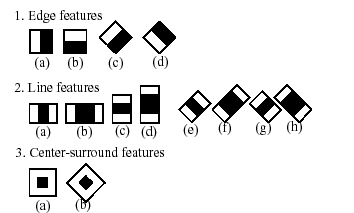
\includegraphics[width=0.8\maxwidth]{../figures/haarfeatures.png}
    \caption{Χαρακτηριστικά τύπου Haar\label{fig:haarfeatures}}
   \end{center}
\end{figure}


Εφαρμόζοντας τον μετασχηματισμό Wavelet με τη συναρτησιακή βάση Haar, προκύπτει
ένας περιορισμένος αριθμός χαρακτηριστικών~\cite{OrePapSinOsu97}. Στο μονοδιάστατο μετασχηματισμό, η
απόσταση ανάμεσα σε δύο γειτονικά κυματίδια (wavelets), σε επίπεδο $n$ , θα είναι $2 n$ . Η απόσταση αυτή είναι
πολύ μεγάλη, κι έτσι δεν λαμβάνουμε όσες πληροφορίες θέλουμε από μια εικόνα ώστε να την
περιγράψουμε λεπτομερώς. Για να έχουμε, λοιπόν, μια πιο λεπτομερή, χωρικά, αναπαράσταση του
περιεχομένου της εικόνας χρειαζόμαστε ένα σύνολο από πλεονάζουσες συναρτήσεις βάσης. Για να
το πετύχουμε αυτό, εφαρμόζουμε τις συναρτήσεις Haar με μεταξύ τους απόσταση ένα
εικονοστοιχείο κάθε φορά. Έτσι, θα έχουμε μια πολύ πιο πυκνή αναπαράσταση. Επίσης, στο
μετασχηματισμό Wavelet, το μέγεθος των συναρτήσεων Haar, κανονικά διπλασιάζεται σε κάθε
επανάληψη. Για να αυξήσουμε ακόμα περισσότερο την λαμβανόμενη πληροφορία από την εικόνα,
ορίζουμε ότι το μέγεθος των συναρτήσεων Haar θα αυξάνει κάθε φορά κατά ένα μόνο
εικονοστοιχείο. Έτσι, το σύνολο των χαρακτηριστικών Haar σε μία εικόνα γίνεται
υπερπολλαπλάσιο του αρχικού. Αυξάνουμε, δηλαδή, την ποσότητα της πληροφορίας που αντλούμε
από μια εικόνα, αυξάνοντας τα χαρακτηριστικά τύπου Haar που θα υπολογιστούν σε αυτήν.

Τα κλασσικά Haar χαρακτηριστικά φαίνονται στο Σχήμα \ref{fig:haarfeatures}.1 (Edge features) ~\cite{OrePapSinOsu97}.
Είναι σχετικά απλά και μπορούν να εντοπίσουν ακμές οριζόντια και κατακόρυφα καθώς και διαγώνιες γραμμές. Για να
μπορέσουμε να αναπαραστήσουμε γραμμές, ράβδους και τετράγωνα καλύτερα, προσθέτουμε τα
χαρακτηριστικά που φαίνονται στο Σχήμα \ref{fig:haarfeatures}.2 (Line features)(τα χαρακτηριστικά iv και v εμφανίζονται στο
~\cite{Viola01rapidobject}, ενώ τα υπόλοιπα στο ~\cite{Lienhart02anextended},
τα οποία υπολογίζονται χωρίς να αυξάνεται ιδιαίτερα η
πολυπλοκότητα, όπως θα δούμε στην ενότητα 2.2. Μια μεγάλη προσθήκη είναι τα χαρακτηριστικά
που είναι περιστραμμένα κατά 45 \degree και φαίνονται στο Σχήμα \ref{fig:haarfeatures}.3 ~\cite{Lienhart02anextended}. Με τη χρήση αυτών
βελτιώνεται σημαντικά η αναπαράσταση των διαγώνιων σχημάτων. Με την προσθήκη όλων αυτών
των χαρακτηριστικών, το σύνολο γίνεται υπερπλήρες και αναπαριστά πολύ καλύτερα την
πληροφορία που περιέχεται σε μία εικόνα.

Για τον υπολογισμό του πλήθους των Haar χαρακτηριστικών σε κάποιο παράθυρο εικόνας
πλάτους W και ύψους H, ακολουθούμε την παρακάτω διαδικασία ~\cite{Lienhart02anextended}. Έστω ότι w και h
είναι το πλάτος και ύψος του ορθογωνίου της συνάρτησης Haar που εξετάζουμε. Το μέγεθος του
ορθογωνίου θα αυξάνεται κατά ένα σε κάθε βήμα. Άρα, οι μέγιστοι συντελεστές μεγέθυνσης των
ορθογωνίων σε πλάτος και ύψος θα είναι $X = \lfloor \frac{W}{w} \rfloor $ και $Y = \lfloor \frac{H}{h} \rfloor$ , αντίστοιχα. Το πλήθος των
χαρακτηριστικών που προκύπτουν από την εφαρμογή ενός κατακόρυφου Haar χαρακτηριστικού
στο παράθυρο εικόνας, είναι:
$$
XY \cdot \Bigg(W+1-w \frac{X+1}{2} \Bigg) \cdot \Bigg(H+1-h \frac{Y+1}{2} \Bigg)
$$

Μπορούμε τώρα να εφαρμόσουμε τους παραπάνω τύπους για ένα παράθυρο μεγέθους 30x30.
Τότε θα έχουμε $W=20$ και $Η=20$ και το πλήθος των χαρακτηριστικών στο παράθυρο φαίνεται
στον παρακάτω πίνακα ~\ref{tab:haarsum}:


\begin{table}[htbp]
  \centering
    \begin{tabular}{ | l | l | l | l | l | l | }
    \hline
        χαρακτηριστικό  & w & h  & X  & Y & πλήθος \\ \hline
    \hline
        t  & 2 & 1 & 10 & 20 & 21.000 \\
    \hline
        & 1 & 2 & 20 & 10 & 21.000 \\
    \hline
        & 2 & 2 & 10 & 10  & 10.000\\
    \hline
        & 3 & 1 & 6 & 20 & 13.230 \\
    \hline
        & 1 & 3 & 20 & 6 & 13.230 \\
    \hline
        & 4 & 1 & 5 & 20 & 9.450\\
    \hline
        & 1 & 4 & 20 & 5 & 9.450\\
    \hline
        & 3 & 3 & 6 & 6 & 3.969 \\
    \hline
        & 1 & 2 & 6 & 6 & 3.969\\
    \hline
        & 2 & 1 & 6 & 6 & 3.969\\
    \hline
        & 3 & 1 & 5 & 5 & 2.025 \\
    \hline
        & 1 & 3 & 5 & 5 & 2.025 \\
    \hline
        & 4 & 1 & 4 & 4 & 1.156 \\
    \hline
        & 1 & 4 & 4 & 4 & 1.156 \\
    \hline
        & 3 & 3 & 3 & 3 & 729 \\
    \hline
        Σύνολο & & & & &116.358 \\
    \hline
  \end{tabular}
  \caption{Πλήθος χαρακτηριστικών Haar ανά παραάθυρο}
  \label{tab:haarsum}
\end{table}

Αυτό που παρατηρούμε είναι ότι σε ένα παράθυρο μεγέθους 20x20 δηλαδή 400 pixel
μπορούν να υπολογιστούν 116.358 χαρακτηριστικά. To πλήθος αυτό είναι
εντελώς δυσανάλογο με τον αριθμό των pixel σε εκείνο το παράθυρο.
Η εξήγηση είναι ότι το σύνολο των χαρακτηριστικών που εξετάσαμε είναι υπερπλήρες
για την περιγραφή ενός παραθύρου.
Στη συνέχεια θα δούμε πως μπορούμε να υπολογίσουμε τα χαρακτηριστικά αυτά
πολύ γρήγορα (σε γραμμικό χρόνο) με τη βοήθεια του ολοκληρώματος εικόνας (Integral Image)

\subsection{Ολοκλήρωμα εικόνας}

Όπως είδαμε το πλήθος των χαρακτηριστικών για ένα παράθυρο 20x20 είναι περίπου 120.000.
Για να υπολογίσουμε ένα χαρακτηριστικό ο προφανής τρόπος είναι να αθροίσουμε τις
τιμές των pixel που απαρτίζουν κάθε ορθογώνιο. Ένας τέτοιος υπολογισμός όμως για 120.000
χαρακτηριστικά είναι αρκετά χρονοβόρος. Σε αυτη την περιπτωση μπορουμε να χρησιμοποιησουμε
μια ενδιαμεση αναπαρασταση της εικονας, το ολοκληρωμα εικονας (\emph{Integral Image})
\footnote{Στη βιβλιογραφία συχνά αναφέρεται και ως Πίνακας Προστιθέμενου Εμβαδού (
Summed Area Table)}
~\cite{Lienhart02anextended}~\cite{Lienhart2003}.
Χρησιμοποιωντας το ολοκληρωμα εικονας μπορουμε να υπολογισουμε καθε Haar feature
σε σταθερο χρονο.

Yπολογίζουμε το ολοκλήρωμα εικόνας σε ένα συγκεκριμένο σημείο $(x,y)$
χρησιμοποιώντας την ακόλουθη σχέση:
$$
ii(x,y) = \displaystyle\sum_{x'\leq x, y'\leq y} i(x',y')
$$

όπου $ii(x,y)$ είναι η τιμή του ολοκληρώματος εικόνας και $i(x,y)$ είναι η τιμή
της πραγματικής εικόνας (δλδ η τιμή χρώματος του εικονοστοιχείου )στο σημείο $(x,y)$.
Ουσιαστικά η τιμή $ii(x,y)$ είναι το άθροισμα των τιμών των εικονοσοιχείων που
βρίσκονται από πάνω και αριστερά του σημείου $(x,y)$.

Χρησιμοποιώντας τις ακόλουθες σχέσεις:
$$
s(x,y) = s(x,y-1) + i(x,y) \hspace{1cm} (1)
$$
$$
ii(x,y) = ii(x-1,y) + s(x,y) \hspace{1cm} (2)
$$
(όπου $s(x,y)$ είναι το άθροισμα των στοιχείων (pixel) μιας γραμμής και $s(x, -1)=0, ii(-1,y)=0$)
καταλήγουμε στη σχέση:

$$
ii(x,y) = i(x,y) + ii(x,y-1) + ii(x-1,y) - ii(x-1,y-1)
$$

Μπόρουμε λοιπόν να υπολογίσουμε το ολοκλήρωμα εικόνας για όλα τα σημεία σε γραμμικό
χρόνο κάνοντας μόνο ενα πέρασμα απο όλα τα στοιχεία της εικόνας.

%Να μπει εδώ εικόνα για Integral Image & Rotated Integral Image
%Να μπει εδώ εικόνα για τρόπο υπολογισμού του αθροίσματος ενός ορθογωνίου
\begin{figure}[htbp]
  \begin{center}
    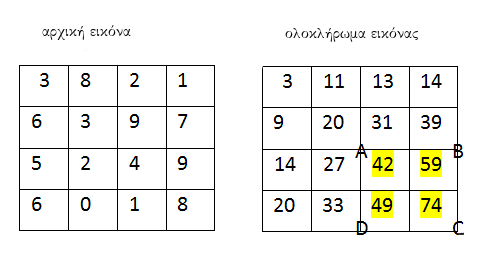
\includegraphics[width=1.0\maxwidth]{../figures/integrimgr3.png}
    \caption{Υπολογισμός ολοκληρώματος εικόνας\label{fig:integrimg}}
   \end{center}
\end{figure}


Αν το δούμε σχηματικά, εχοντας το Ολοκλήρωμα Εικόνας (Integral Image), κάθε κάθετο ορθογώνιο
πάνω στην εικόνα μπορεί να υπολογιστεί χρησιμοποιώντας
4 αναφορές στον πίνακα (βλ Σχήμα \ref{fig:integrimg}). Αντίστοιχα, η διαφορά μεταξύ
δύο ορθογωνίων μπορεί να υπολογιστεί με 8 αναφορές στον πίνακα. Παρακάτω θα δούμε
πως αυτά εφαρμόζονται για τον υπολογισμό των χαρακτηριστικών τύπου Haar σε σταθερό
χρόνο με όσο το δυνατόν λιγότερες πράξεις. Παραδείγματος χάρη από το Σχ. \ref{fig:integrimg}
$$
S_{ABCD} = ii_{C} + ii_(A) - ii_(B) - ii_(D)
$$

Το περιστραμμένο κατά 45\degree ολοκλήρωμα  εικόνας ~\cite{Lienhart02anextended}
~\cite{Lienhart2003} στη θέση $(x,y)$ περιλαμβάνει
το άθροισμα των τιμών όλων των στοιχείων (pixel) που βρίσκονται στο περιστραμμένο
κατά 45\degree ορθογώνιο που έχει το κατώτερο σημείο του στο σημείο $(x,y)$
(βλ Σχήμα \ref{fig:rotintegrimg}). Έτσι το 45\degree Rotated Integral Image ορίζεται ως:
$$
rii(x,y) = \displaystyle\sum_{y'\leq y, y'\leq y-|x-x'|} i(x',y')
$$

Αντίστοιχα χρησιμοποιώντας τις σχέσεις:
$$
rii(x,y) = rii(x-1,y-1) + rii(x+1,y-1) - rii(x,y-2) + i(x,y) + i(x,y-1)
$$
και
$$
rii(-1,y)=rii(x,-1)=rii(x,-2)=rii(-1,-1)=rii(-1,-2)=0
$$

μπορουμε να υπολογισουμε τον πινακα περιστραμμενου προστιθεμενου εμβαδου με ενα
περασμα ολων των στοιχειων της εικονας, απο αριστερα προς τα δεξια και απο πανω
προς τα κατω.

\begin{figure}[htbp]
  \begin{center}
    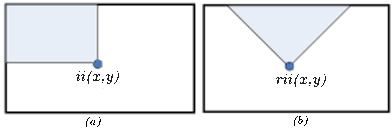
\includegraphics[width=1.0\maxwidth]{../figures/rotintegrimg2.png}
    \caption{Υπολογισμός 45\degree-περιστραμένου ολοκληρώματος εικόνας\label{fig:rotintegrimg}}
   \end{center}
\end{figure}

Επομενως οπως μπορουμε να καταλαβουμε και απο το Σχημα \ref{fig:rotintegrimg}
 για να υπολογισουμε το εμβαδον ενος περιστραμμενου ορθογωνιου εντος μιας εικονας
 χρειαζομαστε μονο 4 αναφορες στον ανωτερο πινακα, και αρα σταθερο χρονο.

Ας εφαρμοσουμε ομως ολη την παραπανω λογικη για να υπολογίσουμε ένα χαρακτηριστικό
τύπου Haar.

Ας δούμε τώρα, το κόστος υπολογισμού κάθε χαρακτηριστικού που χρησιμοποιούμε, με
χρήση του ολοκληρώματος εικόνας. Για τον υπολογισμό των χαρακτηριστικών που αποτελούνται από
δύο γειτονικά ορθογώνια (από τον Πίνακα \ref{tab:haarsum} τα i, ii, ix, x) θα χρειαστούμε 6 αναφορές σε πίνακα
και 6 αριθμητικές πράξεις για τον υπολογισμό των δύο ορθογωνίων και 1 αριθμητική πράξη για τη
μεταξύ τους αφαίρεση. Άρα, συνολικά 6 αναφορές σε πίνακα και 7 αριθμητικές πράξεις. Για τον
υπολογισμό των χαρακτηριστικών που αποτελούνται από τρία γειτονικά ορθογώνια (από  τον Πίνακα
\ref{tab:haarsum} τα iv-vii, xi-xiv) θα χρειαστούμε 8 αναφορές σε πίνακα και 11 αριθμητικές πράξεις (9 για τον
υπολογισμό των ορθογωνίων και 2 για τις μεταξύ τους πράξεις). Οι πράξεις τελικά μειώνονται σε 8
ακολουθώντας το σκεπτικό που φαίνεται στον Πίνακα \ref{tab:opthaar} ~\cite{Lienhart02anextended}. Τα χαρακτηριστικά viii και xv
που φαίνονται στον Πίνακα \ref{tab:haarsum}, παρότι αποτελούνται από δύο ορθογώνια, αυτά δεν είναι γειτονικά
μεταξύ τους. Έτσι, για τον υπολογισμό τους, σύμφωνα με τον Πίνακα \ref{tab:opthaar}, χρειάζονται 8 αναφορές
σε πίνακα και 8 αριθμητικές πράξεις. Για το χαρακτηριστικό iii που αποτελείται από τέσσερα
ορθογώνια, απαιτούνται 9 αναφορές σε πίνακα και 12 αριθμητικές πράξεις. Βλέπουμε, λοιπόν, ότι
όλα τα χαρακτηριστικά που περιγράφηκαν στην ενότητα 2.2.1 μπορούν να υπολογιστούν σε σταθερό
χρόνο, ανεξάρτητα από το μέγεθος του χαρακτηριστικού, με τη χρήση των δύο αυτών πινάκων. Το
γεγονός αυτό, επιταχύνει δραστικά το σύστημα ανίχνευσης.


\begin{table}[htbp]
  \centering
    \begin{tabular}{ | l | l | }
    \hline
        χαρακτηριστικό  & 3 ορθογώνια $\rightarrow$ 8 αναφορές και 11 πράξεις \\
    \hline
        t  & 2 ορθογώνια $\rightarrow$ 8 αναφορές και 6 πράξεις \\
    \hline
       t &  8 αναφορές και 8 πράξεις \\
    \hline
  \end{tabular}
  \caption{Μείωση του κόστους υπολογισμού χαρακτηριστικών με 3 ορθογώνια}
  \label{tab:opthaar}
\end{table}


Η ανίχνευση αντικειμένων, θα πρέπει να γίνει σε κάθε δυνατή θέση της εικόνας, καθώς επίσης
και σε κάθε δυνατή κλίμακα. Για τον έλεγχο σε κάθε θέση, ο ανιχνευτής κινείται μέσα στην εικόνα,
διατρέχοντάς την ολόκληρη, και εφαρμόζοντας τη μέθοδο ανίχνευσης σε κάθε υποπαράθυρο. Για
τον έλεγχο σε κάθε κλίμακα, άλλες μέθοδοι δημιουργούν μια πυραμίδα από σμικρύνσεις της
εικόνας, και εφαρμόζουν σε κάθε κλίμακα της πυραμίδας τον ανιχνευτή, διατηρώντας σταθερό το
μέγεθός του. Με αυτή τη μέθοδο, πέρα από το κόστος της ίδιας της ανίχνευσης, προστίθεται και
το χρονικό κόστος της κατασκευής της πυραμίδας εικόνων, το οποίο είναι αρκετά σημαντικό. Στη
μέθοδο που εξετάζουμε, αντί να αλλάζουμε το μέγεθος της εικόνας όπου γίνεται η ανίχνευση,
αλλάζουμε το μέγεθος του ίδιου του ανιχνευτή. Αυτό είναι εφικτό, καθώς τα χαρακτηριστικά τύπου
Haar μπορούν να μεταβληθούν σε μέγεθος. Επίσης, με τη χρήση των δύο πινάκων που είδαμε
προηγουμένως, ο υπολογισμός ενός χαρακτηριστικού δεν επηρεάζεται χρονικά από το μέγεθός
του. Έτσι, η εφαρμογή της μεθόδου μπορεί να γίνει στον ίδιο ακριβώς χρόνο για οποιαδήποτε
κλίμακα του παραθύρου ανίχνευσης. Από μετρήσεις που έχουν γίνει, έχει βρεθεί ότι ο χρόνος που
χρειάζεται για την κατασκευή της πυραμίδας εικόνων που χρησιμοποιούν άλλες μέθοδοι, είναι
παραπλήσιος με το χρόνο που χρειάζεται η μέθοδος που εξετάζουμε, για όλη τη διαδικασία
ανίχνευσης [ViJo02]. Έτσι, βλέπουμε ότι οποιαδήποτε μέθοδος χρησιμοποιεί πυραμίδες εικόνων
για την ανίχνευση αντικειμένων, θα είναι αναγκαστικά πιο χρονοβόρα από την εξεταζόμενη
μέθοδο.

\subsection{Ο αλγόριθμος AdaBoost}

Στην προηγούμενη ενότητα παρουσιάσαμε τo σύνολο των Haar features. Tα χαρακτηριστικά
αυτά μας βοηθούν να δούμε αν στο τρέχον παράθυρο
εντός της εικόνας που εξετάζουμε υπάρχει κάποιο αντικέιμενο (στη συγκεκριμένη
περίπτωση πρόσωπο). Μας βοηθάνε δηλαδή να \emph{ταξινομίσουμε} τα επιμέρους παράθυρα
επιλέγοντας εκείνα που περιέχουν πρόσωπα. Η διαδικασία αυτή ονομάζεται ταξινόμηση
(\emph{Classification}) και ο αλγόριθμος που υλοποιει, ταξινομητης (\emph{Classifier}).

Όπως είδαμε, τα χαρακτηριστικά που χρησιμοποιούμε μπορούν να υπολογιστούν πάρα πολύ
γρήγορα. Το σύνολο όμως των χαρακτηριστικών παραμένει μεγάλο (περίπου 120.000 για μια
εικόνα 20x20).Συνεπως, η διαδικασία υπολογισμού του συνόλου των χαρακτηριστικών
για όλα τα παράθυρα μέσα σε μια εικόνα παραμένει κοστοβόρα ~\cite{Viola01rapidobject}.
Χρειάζεται λοιπόν, να επιλέξουμε ένα υποσύνολο των χαρακτηριστικών αυτών τα υποία θα
είναι ικανά να μας παρέχουν την πληροφορία για την ύπαρξη αντικειμένου.

Ο αλγόριθμος AdaBoost ειναι ενας αλγοριθμος μηχανικης μαθησης ο οποιος χρησιμοποιειται
τοσο για την επιλογη του υποσυνολου των χαρακτηριστικων που θα χρησιμοποιηθουν
απο τον classifier, οσο και για την εκπαιδευση του ταξινομητη. Ανηκει στην κατηγορια
των boosting algorithms, χρησιμοποιειται δηλαδη για να αυξησει την αποδοση ενος
οποιουδηποτε απλου αλγοριθμου ταξινομησης (\emph{weak classifier}). Στην πραγματικότητα,
αυτό που κάνει ο AdaBoost είναι να φτιάξει μια αλυσίδα από από weak classifiers
χρησιμοποιώντας ένα άπληστο αλγόριθμο, ώστε να σχηματίσει τελικά από αυτούς έναν
ισχυρότερο classifier.

Η βελτίωση του ασθενούς αλγορίθμου ταξινόμησης πραγματοποιείται, καλώντας τον
αλγόριθμο να επιλύσει μια αλληλουχία προβλημάτων ταξινόμησης. Αρχικά, όλα τα παραδείγματα
(θετικά και αρνητικά) παίρνουν μια τιμή βάρους, η οποία είναι ίδια για όλα. ∆ίνονται στον
αλγόριθμο και πραγματοποιείται ο πρώτος κύκλος εκμάθησης, όπου ο
αλγόριθμος ταξινομεί όλα τα παραδείγματα με κάθε διαθέσιμη συνάρτηση ταξινόμησης. Έπειτα,
οι συναρτήσεις ταξινόμησης διατάσσονται σύμφωνα με τα αποτελέσματά τους, λαμβάνοντας υπόψη
το βάρος κάθε παραδείγματος. Επιλέγεται ένας μικρός αριθμός συναρτήσεων ταξινόμησης, από
αυτές με τα καλύτερα αποτελέσματα, που αποτελούν τον πρώτο ασθενή ταξινομητή. Ο πρώτος
κύκλος εκμάθησης ολοκληρώνεται και τα βάρη των παραδειγμάτων ισοσταθμίζονται, δίνοντας
μεγαλύτερο βάρος στα παραδείγματα που ταξινομήθηκαν λανθασμένα από τον πρώτο ασθενή
ταξινομητή. Έτσι, στον δεύτερο κύκλο εκμάθησης ο αλγόριθμος ταξινόμησης θα θεωρήσει πιο
σημαντικά τα παραδείγματα που ταξινομήθηκαν λανθασμένα από τον προηγούμενο ταξινομητή.
Τα βήματα επαναλαμβάνονται διαδοχικά, μέχρι να φτάσουμε στο επίπεδο του συνολικού λόγου
λανθασμένης ταξινόμησης που επιθυμούμε. Τελικά, ο ισχυρός ταξινομητής προκύπτει από τον
συνδυασμό των ασθενών ταξινομητών που επιλέχθηκαν και ένα κατώφλι. Κατά την διαδικασία της
ταξινόμησης ενός υποπαραθύρου εικόνας από τον ισχυρό ταξινομητή, εφαρμόζονται στο
υποπαράθυρο όλοι οι ασθενείς ταξινομητές. Τα αποτελέσματα των ασθενών ταξινομητών
αθροίζονται, και αν το άθροισμα ξεπερνά το κατώφλι του ταξινομητή, το υπό εξέταση αντικείμενο
ταξινομείται ως θετικό, αλλιώς ως αρνητικό.

%------

Ο αλγόριθμος AdaBoost διαθέτει 4 διαφορετικές εκδοχές ~\cite{Friedman98additivelogistic}.
Η αρχική εκδοχή ονομάζεται ∆ιακριτός AdaBoost (\emph{Discrete AdaBoost - DAB}) καθώς η συνάρτηση ταξινόμησης
κάθε weak classifier παίρνει 2 διακριτές τιμές ${-1,1}$ ανάλογα με το αν ένα
δείγμα ταξινομείται ως θετικό ή αρνητικό. Η δεύτερη εκδοχή ονομάζεται Πραγματικός AdaBoost
(\emph{Real AdaBoost - RAB}), καθώς η συνάρτηση ταξινόμησης έχει ως πεδίο τιμών ολόκληρο
το διάστημα $[0,1]$. Με τη χρήση του RAB, μπορούμε να έχουμε μια
ένδειξη εμπιστοσύνης για τα αποτελέσματα της ταξινόμησης, χρησιμοποιώντας τις τιμές που
επιστρέφονται από τον αλγόριθμο και όχι μόνο το αποτέλεσμα της θετικής ή αρνητικής
ταξινόμησης. Άλλη εκδοχή είναι ο LogitBoost, ο οποίος έχει δύο παραλλαγές, αυτή που
χρησιμοποιεί δύο κλάσεις και αυτή που χρησιμοποιεί J κλάσεις
Τέλος υπάρχει και ο Gentle AdaBoost, οποίος ουσιαστικά βασίζεται στον Real AdaBoost
παράγει όμως τα επιμέρους βήματα χρησιμοποιώντας τη μέθοδο Newton αντί να χρησιμοποιεί
ακριβή υπολογισμό σε κάθε βήμα.

Στη μέθοδο που χρησιμοποιησαμε για την ανιχνευση προσωπων, κάθε ασθενής αλγόριθμος
εκμάθησης παραγει τιμες απο το περιορισμενο συνολο συναρτησεων ταξινομησης που αποτελούνται από ένα
μόνο χαρακτηριστικό τύπου Haar. Προφανώς, από ένα μόνο χαρακτηριστικό δε μπορούμε να
περιμένουμε ιδιαίτερα χαμηλό λόγο σφάλματος. Σε κάθε στάδιο του αλγορίθμου AdaBoost
επιλέγεται το χαρακτηριστικό που διαχωρίζει καλύτερα τα θετικά από τα αρνητικά δείγματα. Για
κάθε χαρακτηριστικό, ο weak classifier προσδιορίζει ένα κατώφλι της τιμής του
χαρακτηριστικού, που ελέγχοντάς το περιορίζονται οι λανθασμένες ταξινομήσεις από το
συγκεκριμένο χαρακτηριστικό στις ελάχιστες δυνατές. Έπειτα, επιλέγεται ως ασθενής ταξινομητής
το χαρακτηριστικό τύπου Haar, που, για το δεδομένο κατώφλι του, κάνει τη συνολικά καλύτερη
ταξινόμηση. Ο AdaBoost συνεχίζει εκπαιδεύοντας όλους τους ασθενείς ταξινομητές, μέχρι το
σημείο που ο ισχυρός συνολικός ταξινομητής επιτυγχάνει το επίπεδο ταξινόμησης που ζητάμε.

Ο αλγόριθμος AdaBoost παρέχει αρκετά ισχυρές εγγυήσεις για την ορθότητά του. Έχει
αποδειχθεί, ότι το σφάλμα ταξινόμησης του ισχυρού ταξινομητή που προκύπτει από την εφαρμογή
του αλγορίθμου, τείνει προς το μηδέν εκθετικά ως προς τον αριθμό των κύκλων εκπαίδευσης
~\cite{schapire1998}. Εξίσου σημαντικό αποτελεί το γεγονός ότι η όλη διαδικασία της
εκμάθησης πραγματοποιείται  σχεδόν σε πραγματικό χρόνο.
Για να κατασκευάσουμε έναν Classifier από τον αλγόριθμο AdaBoost με Μ επιμέρους
Weak Classifiers από ένα συγκεκριμένο πλήθος Κ χαρακτηριστικών Haar για Ν εικόνες
χρειαζόμαστε χρόνο $O(MKN)$. Αντίθετα άλλοι αλγόριθμοι χρειάζονται $O(MNKN)$ βήματα.

\subsection{Χρήση ενός Cascade Classifier}

Σε αυτή την ενότητα παρουσιάζεται η μέθοδος ταξινόμησης εικόνων με τη χρήση ενός
Cascade Classifier ~\cite{Viola01rapidobject}. Η μέθοδος αυτή βοηθά στη επίτευξη υψηλού λόγου
ανίχνευσης, μειώνοντας σημαντικά τον απαιτούμενο χρόνο. Η γενική ιδέα είναι ότι αντί για
έναν μεγάλο και χρονοβόρο classifier μπορούμε να χρησιμιποιήσουμε διαδοχικά πολλούς
μικρότερους (άρα και γρηγορότερους) classifiers. Στη συγκεκριμένη περίπτωση χρησιμοποιούμε
απλούστερους και πολύ γρήγορους ταξινομητές (ελέγχουν λιγότερα haar features) αρχικά,
οι οποίοι θα απορρίπτουν γρήγορα την πλειονότητα των αρνητικών υποπαραθύρων,
και πιο σύνθετους και χρονοβόρους που ελέγχουν περισσότερα haar features αργότερα ,
ώστε να μειώσουμε το λόγο λανθασμένων ανιχνεύσεων.

Κάθε υποπαράθυρο της εικόνας εισέρχεται στον πρώτο ταξινομητή. Αν ο ταξινομητής το κατατάξει ως
θετικό, αυτό περνά ως είσοδος στον δεύτερο ταξινομητή. Αν και αυτός το κατατάξει ως θετικό,
τότε περνά στον τρίτο κ.ο.κ. Αν σε αυτή τη διαδοχή κάποιος ταξινομητής κατατάξει το
υποπαράθυρο ως αρνητικό, τότε αυτό απορρίπτεται και δεν εξετάζεται από κανένα άλλο
ταξινομητή (βλέπε Σχήμα \ref{fig:cascadeclassifier}). Θα μπορούσαμε να παρομοιάσουμε
αυτή τη διαδικασία με έναν μεγάλο ταξινομητή που αποτελείται από το σύνολο των χαρακτηριστικών
Haar, όπου όμως δεν περιμένουμε να υπολογιστεί όλο το πλήθος των χαρακτηριστικών.
Αντίθετα, σε κάθε στάδιο ελέγχονται μερικά χαρακτηριστικά και ανάλογα με το άθροισμα
των τιμών τους ο ταξινομητής αποφασίζει αν το υπο εξέταση υποπαράθυρο απορρίπτεται ή όχι.

\begin{figure}[htbp]
  \begin{center}
    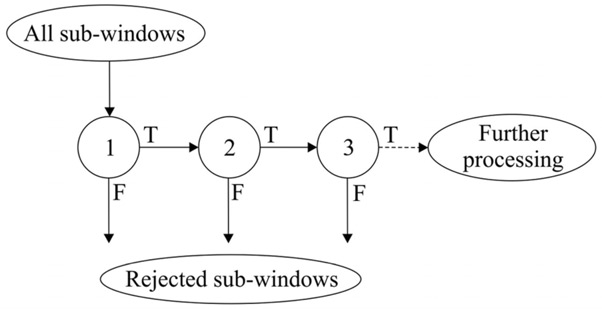
\includegraphics[width=0.5\maxwidth]{../figures/cascadeclassifier.png}
    \caption{Τα επιμέρους βήματα ενός Cascade Classifier\label{fig:cascadeclassifier}}
   \end{center}
\end{figure}

Κάθε ταξινομητής του Cascade Classifier εκπαιδεύεται χρησιμοποιώντας ένα σύνολο θετικών και ένα
σύνολο αρνητικών παραδειγμάτων. Το σύνολο των θετικών παραδειγμάτων είναι το ίδιο
κατά την εκπαίδευση κάθε ταξινομητή. Το σύνολο των αρνητικών παραδειγμάτων όμως,
μεταβάλλεται. Συγκεκριμένα, κάθε ταξινομητής εκπαιδεύεται χρησιμοποιώντας ως
αρνητικά παραδείγματα, τα παραδείγματα που ταξινομούνται από τους προηγούμενους ταξινομητές
ως θετικά ~\cite{Viola01rapidobject}. Αυτό αυξάνει σε πολύ μεγάλο βαθμό τα
αρνητικά παραδείγματα τα οποία θα εξεταστούν συνολικά. Για να φτάσει ένας συγκεκριμένος
αριθμός αρνητικών παραδειγμάτων στον τρέχοντα ταξινομητή, θα πρέπει τα παραδείγματα αυτά
να ταξινομηθούν από όλους τους προηγούμενους ταξινομητές (λανθασμένα) ως θετικά.
Ας θεωρήσουμε ότι σε κάθε στάδιο ενός Cascade Claasifier θέλουμε να εξετάζονται 1.000 αρνητικά
παραδείγματα και κάθε στάδιο έχει λόγο λανθασμένης θετικής ανίχνευσης 0,5. Τότε, για να
περάσουν στο δέκατο στάδιο 1.000 αρνητικά παραδείγματα, αυτά θα χρειαστεί να έχουν
ταξινομηθεί από τα προηγούμενα εννιά στάδια ως θετικά. Έτσι, συνολικά θα πρέπει να εξεταστούν
περίπου 512.000 αρνητικά παραδείγματα.

Η εξέταση πολύ μεγαλύτερου αριθμού αρνητικών παραδειγμάτων αυξάνει την τελική απόδοση
του CC. Αντίθετα, κάθε ταξινομητής καλείται να πραγματοποιήσει μια πιο δύσκολη ταξινόμηση
από αυτές των προηγούμενων ταξινομητών. Τα αρνητικά παραδείγματα που θα έχει στη διάθεσή
του θα είναι πιο δύσκολα στην ταξινόμηση από τα παραδείγματα που είχαν τα προηγούμενα από
αυτό στάδια. Έχοντας, λοιπόν, πιο δύσκολο σύνολο εκπαίδευσης ένας ταξινομητής που βρίσκεται
σε προχωρημένο στάδιο, θα παρουσιάσει αυξημένες λανθασμένες ταξινομήσεις, θετικές και
αρνητικές.

Οι απλοί επιμέρους ταξινομητές, θα πρέπει να έχουν πολύ χαμηλό λόγο λανθασμένων
αρνητικών ταξινομήσεων, ώστε να μην χάνονται τα πραγματικά αντικείμενα στη συνολική
ταξινόμηση. Για να διασφαλίσουμε τη σωστή λειτουργία του CC, θα πρέπει να αυξήσουμε
περαιτέρω τις θετικές ταξινομήσεις (είτε αφορούν πραγματικά αντικείμενα είτε όχι)
~\cite{Viola01rapidobject}. Μια τεχνική για να πετύχουμε αυτό το αποτέλεσμα είναι
να επέμβουμε στις τιμές των κατωφλίων των ταξινομητών που προσδιόρισε ο αλγόριθμος
AdaBoost κατά την εκπαίδευση. Το κατώφλι ενός ταξινομητή ορίζει την ελάχιστη τιμή
του σταθμισμένου με βάρη αθροίσματος των τιμών των χαρακτηριστικών που θα πρέπει
να έχει ένα υποπαράθυρο για να ταξινομηθεί ως θετικό. Ένα υποπαράθυρο ταξινομείται,
δηλαδή, ως θετικό, όταν το (σταθμισμένο) άθροισμα των τιμών των χαρακτηριστικών που
υπολογίστηκαν για αυτό ξεπερνά το κατώφλι του ταξινομητή. Έτσι, μειώνοντας τις
τιμές των κατωφλίων θα αυξηθεί ο αριθμός των παραθύρων που ταξινομούνται ως
θετικά, άρα και ο λόγος θετικών ταξινομήσεων.

Ο ολοκληρωμένος CC που χρησιμοποιήθηκε για την ανίχνευση προσώπων αποτελείται
από 38 επιμέρους στάδια και ένα σύνολο 6000 χαρακτηριστικών. Ο χρόνος που
απαιττείται για να τρέξει ο CC είναι άμεσα συνδεδεμένος με τον συνολικό αριθμό των
χαρακτηριστικών που υπολογίζονται για κάθε υποπαράθυρο που εξετάζεται.
Με βάση αξιολογήσεις που έχουν γίνει ~\cite{Viola01rapidobject}~\cite{Viola2004}
πάνω στο MIT-CMU test set ~\cite{Rowley:1998:NNF:275341.275344} υπολογίζονται κατά
μέσο όρο 10 Haar features από τα συνολικά 6061 ανά υποπαράθυρο. Αυτό οφείλεται
στο γεγονός ότι το μεγαλύτερο ποσοστό από τα υποπαράθυρα απορρίπτεται σε πρώτα
στάδια.

Η απόδοση του CC εξαρτάται επίσης από το πλήθος των επιμέρους σταδίων και την
απόδοση του καθενός από αυτά.


\section{Άλλες μέθοδοι που έχουν χρησιμοποιηθεί}\label{sec:othermethods}

Στο κεφάλαιο αυτό κάναμε μισ σύντομη αναφορά στις πιο βασικές μεθόδους αναγνώρισης
πρσώπου σε εικόνα με βάση την απόδοση που επιτυγχάνουν και το χρόνο εκτέλεσής τους.
Οι τεχνικές αυτές βασίζονται κατά κύριο λόγο στον υπολογισμό κάποιων χαρακτιρηστικών
σκίασης από την εικόνα σε συνδιασμό με κάποιο προεκπαιδευμένο μοντέλο αναγνώρισης.
Γενικά, στο επιστημονικό πεδίο αυτό έχουν προταθεί αρκετές μέθοδοι με βάση διαφορετικά
χαρακτηριστικά της εικόνας. Μερικά από αυτά είναι το χρώμα, η κίνηση καθώς και
συνδιασμός αυτών. Ενδεικτικά αναφέρουμε μερικές τεχνικές.

\newpage
Τεχνικές σε ελεγχόμενο περιβάλλον (πχ μονοχρωματικό φόντο)
\begin{description}
  \item[Με βάση το χρώμα] \hfill \\
    \begin{itemize}
        \item Explanation of basic color extraction for face detection
            \flink{http://web.archive.org/web/20040815172250/http:/www.dcs.qmul.ac.uk/research/vision/publications/papers/bmvc97/node2.html}
        \item Face detection in color images using PCA
            \flink{http://web.archive.org/web/20070621092425/http:/www.ient.rwth-aachen.de/forschung/bebi/facedetection/publi/men99b.pdf}
    \end{itemize}
  \item[Με βάση την κίνηση] \hfill \\
    \begin{itemize}
        \item Explanation of basic motion detection for face finding
            \flink{http://web.archive.org/web/20080522171806/http:/www.ansatt.hig.no/erikh/papers/hig98_6/node2.html}
        \item Blink detection: human eyes are simultaneously blinking
            \flink{http://www-prima.imag.fr/ECVNet/IRS95/node13.html}
    \end{itemize}
  \item[Με συνδιασμό των δυο προηγουμένων] \hfill \\
    \begin{itemize}
        \item A mixture of color and 3D
            \flink{http://people.eecs.berkeley.edu/~trevor/papers/1998-021/}
        \item A mixture of color and background removal
            \flink{http://web.archive.org/web/20030821151710/http:/atwww.hhi.de/blick/Head_Tracker/head_tracker.html}
    \end{itemize}
\end{description}
